\chapter{Na\"ieve legoblokdetectie}
\label{hoofdstuk:2}
In dit hoofdstuk bespreken we twee na\"ieve algoritmes om legoblokken te detecteren. Beide algoritmes zullen via een thresholding operatie de blokken lokaliseren. Vervolgens zal het eerste algoritme de geometrie van een legoblok gebruiken om te bepalen wat de pose is van de legoblok. Het tweede algoritme zal via een 2 dimensionaal grid bepalen waar de blokken zich bevinden.

TODO: OVERZICHT VAN HET HOOFDSTUK

%\section{Evaluatiemethode en implementatie}
%In deze sectie bespreken we eerst kort op welke manier de performantie van beide algoritmes worden ge\"evalueerd. Vervolgens wordt kort overlopen welke machine en welke bibliotheken er zijn gebruikt voor de implementaties van de algoritmes.
%
%\subsection{Evaluatiemethode}
%
%\begin{figure}
%  \centering
%  \includegraphics[width=\linewidth]{img/simpleComplex}
%  \caption{Simpele (links) en complexe scene (rechts) voor performantie evaluatie van na\"ieve blokdetectie.}
%  \label{fig:simple_complex}
%\end{figure}
%
%De performantie van beide algoritmes werden ge\"evalueerd door de tijd op te meten van het volledige lemmingenspel zowel wanneer een eenvoudige scene werd gebouwd als wanneer een complexe scene werd gebouwd. Figuur \ref{fig:simple_complex} toont beide scenes die hiervoor zijn gebruikt. Merk op dat dit scenes zijn die simpel en complex zijn voor deze algoritmes, maw. het zijn scenes die beide algoritmes kunnen detecteren en respectievelijk weinig / veel legoblokken bevatten.
%
%De opmeting gebeurde even lang als een lemming nodig heeft om van begin tot eindpunt te geraken. Aangezien de snelheid gedefinieerd is als 0.5 cm/s en de afstand minimum 23 cm is, duurt de opmeting dus minimum 11.5 seconden. Vervolgens wordt per opgemeten gedeelte het gemiddelde genomen om geen grote uitschieters te hebben.
%
%\subsection{Implementatie}
%De volledige implementatie en experimenten in dit hoofdstuk zijn uitgevoerd op een Sony Xperia Z C6602 met een Qualcomm Quad-core 1.5 GHz Krait processor, Adreno 320 GPU, 2GB RAM en Android 4.4.4 KitKat. Alles werd geprogrammeerd in Java 7 met gebruik van de Cardboard VR SDK van Google voor stereo rendering voor de Google Cardboard en de OpenCV 2.4.9 bibliotheek voor implementaties van computer vision algoritmes.

\section{Blokdetectie op basis van simpele geometrische informatie}
Het eerste na\"ieve blokdetectie algoritme steunt op de geometrie van een legoblok om te bepalen waar legoblokken zich bevinden en wat hun pose is. 

Dit eerste algoritme verloopt in twee delen om uiteindelijk de locatie en pose van een legoblok te bepalen: vinden van de contour van de legoblok en bepalen van de pose van de legoblok uit de contour. Eerst bespreken we deze twee onderdelen in een theoretische sectie, vervolgens wordt uitgelegd hoe het algoritme werd ge\"implementeerd en ten slotte bespreken we de resultaten, performantie en voor-en nadelen van deze methode.

\subsection{Begrippen en algoritme} \label{sec:alg1_begrip}

\subsubsection*{Begrippen}

\textbf{Thresholding} is een operatie die vaak in beeldverwerking wordt gebruikt om twee delen in een afbeelding te scheiden van elkaar (vaak voorgrond en achtergrond). Het resultaat is een binaire afbeelding waarin de achtergrond meestal wordt aangeduid met zwart en de voorgrond met wit.

\textbf{YUV}, \textbf{RGB} en \textbf{HSV} zijn drie verschillende kleurenruimtes die elk op een andere manier kleuren defini\"eren. Bij YUV gebeurt dit door de helderheid (Y) van de kleur te scheiden van twee kleurcomponenten (U en V). In RGB zijn er enkel drie kleurcomponenten waarbij de helderheid dus in deze componenten verwerkt zit. HSV scheidt tint (H), verzadiging (S) en helderheid (V) van elkaar. Omdat HSV drie componenten scheidt die een duidelijk verschillende invloed hebben op de uiteindelijke kleur wordt deze kleurenruimte vaak gebruikt voor kleurthresholding, het is immers eenvoudiger om kleuren van elkaar te scheiden zonder de verzadiging of de helderheid te be\"invloeden.

\textbf{Pinhole model} is het model dat OpenCV gebruikt om 3D punten van een scene te transformeren naar de afbeelding via een perspectieftransformatie. In de algoritmes uit dit hoofdstuk wordt het gebruikt om 2D punten om te zetten naar 3D. Dit is de formule van het pinhole model:
$$
s
\begin{bmatrix}
	u \\ 
	v \\
	1
\end{bmatrix} 
=
\begin{bmatrix}
	f_x & 0 & c_x \\ 
	0 & f_y & c_y \\
	0 & 0 & 1
\end{bmatrix} 
\begin{bmatrix}
	r_{11} & r_{12} & r_{13} & t_1 \\ 
	r_{21} & r_{22} & r_{23} & t_2 \\
	r_{31} & r_{32} & r_{33} & t_3 \\
\end{bmatrix}
\begin{bmatrix}
	X \\ 
	Y \\
	Z \\
	1
\end{bmatrix}
$$
Hierbij is $(u,v)$ het 2D punt, $(X,Y,Z)$ het 3D punt, de eerste matrix in het rechterlid de camera intrinsics matrix (bekomen door camera calibratie), de tweede matrix in het rechterlid is de camera extrinsics matrix (afgeleid uit de ligging van de markers) en $s$, tenslotte, is een schaalfactor. Wanneer de twee cameramatrices bekend zijn kunnen we een 3D punt omzetten in 2D en vice versa. Een belangrijke opmerking hierbij is dat, bij omzetting van 2D naar 3D, wat informatie te kort is (het aantal dimensies verhoogt immers). Deze extra informatie kan worden gegeven in twee vormen: ofwel kennen we de uiteindelijke $Z$ co\"ordinaat, ofwel kennen we de uiteindelijke $X$ en $Y$ co\"ordinaten.

%\subsubsection*{Veronderstellingen}
%In dit algoritme worden enkele veronderstellingen gemaakt. In deze sectie bespreken we kort welke veronderstellingen zijn gemaakt en waarom.
%
%\begin{itemize}
%\item De achtergrond bestaat uit wit en zwart, belangrijk is vooral dat ze geen rode tint bevat. Deze restrictie werd opgelegd omdat we in het algoritme kleurthresholding gebruiken om de rode blokken te scheiden van de achtergrond.
%\item Omdat het algoritme gebruik maakt van kleurthresholding is het ook aangeraden om zo weinig mogelijk schaduw te hebben. Anders kan de contour van de legoblok moeilijk gedetecteerd worden waardoor legoblokken mogelijks slecht worden gedetecteerd. In de resultaten (sectie \ref{sec:algo1_res}) tonen we dat dit werkelijk een probleem is.
%\item De blokken die worden gebruikt zijn steeds balkvormig, geen enkele blok of constructie van blokken mag een hoek bevatten. Dit is belangrijk omdat het algoritme ervan uit gaat dat de contour van een te detecteren legoblok bestaat uit maximaal zes hoekpunten. Dit impliceert ook dat legoblokken elkaar niet mogen aanraken vanuit het standpunt van de camera gezien (tenzij ze in elkaars verlengde liggen).
%\item Zoals hierboven reeds aangehaald gaat het algoritme ervan uit dat de contour van een blok maximaal zes hoekpunten bevat. Dit impliceert dat het algoritme beter werkt wanneer we legoblokken vanuit perspectief zien want dan bestaat de omtrek van een blok uit exact zes hoekpunten.
%\end{itemize}

\subsection{Algoritme}

\subsubsection*{Bepalen van de contour}

Eerst wordt de nieuwe frame van het YUV formaat omgezet naar het HSV formaat. Dit is een erg belangrijke stap vanwege twee redenen: ten eerste kan OpenCV niet werken met het YUV formaat en ten tweede is het HSV formaat (zoals hierboven reeds aangehaald) veruit het eenvoudigste formaat om te gebruiken bij thresholding operaties.

Op de HSV frame wordt vervolgens kleurthresholding toegepast om de legoblokken te scheiden van de wit-zwarte achtergrond. In dit eerste algoritme werd enkel gewerkt met de kleur rood. Experimenteel werd ondervonden dat om rood te scheiden van een wit-zwarte achtergrond de HSV waarden in het volgende interval moeten liggen:
$$ 160 < H < 180; 153 < S < 255; 30 < V < 255$$

TODO: IS CANNY EDGE DETECTIE WEL NODIG, AANGEZIEN WE AL EEN THRESHOLD HEBBEN? %TODO

Contouren worden dan bepaald met behulp van de \texttt{findContours} methode van OpenCV. Deze methode gebruikt het algoritme dat wordt beschreven in~\cite{suzuki1985topological}, het wordt hier niet besproken omdat dit out of scope van deze thesis is.

In de volgende stap wordt deze contour benadert met behulp van de \texttt{approxPolyDP} methode van OpenCV. Deze methode benadert deze contours met een polygon. Deze stap is nodig omdat een contour uit een enorme hoeveelheid punten bestaat, na deze benadering blijven de belangrijkste punten over: de hoekpunten van de legoblok. Deze methode bevat een parameter $\epsilon$ die aangeeft wat de maximale afwijking mag zijn van de benadering ten opzichte van de oorspronkelijke contour. Om ervoor te zorgen dat we een zo goed mogelijke benadering verkrijgen in alle gevallen, maken we $\epsilon$ steeds groter tot we net een maximum van zes hoekpunten hebben bereikt. Deze adaptieve techniek behoudt de kwaliteit van de contour maar in ruil daarvoor moeten we de veronderstelling maken dat de omtrek van de contour van de threshold bestaat uit maximaal zes hoeken.

Nu kan het zijn dat er contours zijn met een te kleine oppervlakte door ruis in de kleurthreshold. Om deze te verwijderen bekijken we de oppervlakte van alle contours en worden contours verwijderd met een oppervlakte die 100x kleiner is dan de oppervlakte van de grootste contour.

Het bepalen en verfijnen van de contour is afgelopen, nu moet bepaald worden wat de pose is van de legoblok. Dat gebeurt in het tweede deel van het algoritme.

\subsubsection*{Bepalen van de pose}



\begin{figure}
  \centering
%  \includegraphics[width=0.5\linewidth]{img/brickPoseDetect}
  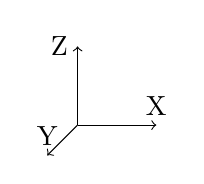
\begin{tikzpicture}
    \draw[->] (0,0,0) -- (0,0,1) node[above]{Y};
    \draw[->] (0,0,0) -- (0,1,0) node[left]{Z};
    \draw[->] (0,0,0) -- (1,0,0) node[above]{X};
  \end{tikzpicture}
  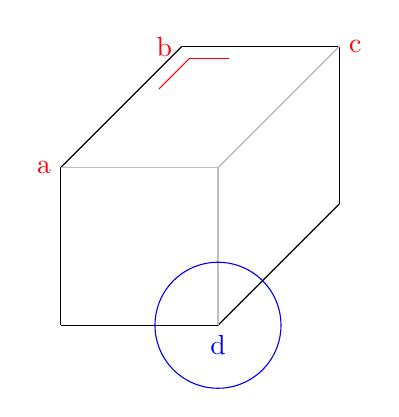
\begin{tikzpicture}
	\draw[black] (0,0 ,4) -- (2,0,4);
    \draw[black] (0 ,0,4) -- (0 ,2,4);
    \draw[black] (2,0 ,4) -- (2,0 ,0);
    \draw[black] (0 ,2,4) node[red,left]{a} -- (0 ,2,0);
    \draw[black] (2,0,0 ) -- (2,2,0 ) node[red,right]{c};
    \draw[black] (0,2,0 ) node[red,left]{b} -- (2,2,0 );
    
    \draw[lightgray] (0,2 ,4) -- (2,2 ,4);
    \draw[lightgray] (2 ,0,4) -- (2 ,2,4);
    \draw[lightgray] (2,2 ,4) -- (2,2 ,0);
    \draw[lightgray] (2 ,2,4) -- (2 ,2,0);
    \draw[lightgray] (2,0,4 ) -- (2,2,4 );
    \draw[lightgray] (0,2,4 ) -- (2,2,4 );
    
	\draw[red] (0.25,2 ,0.40) -- (0.75,2 ,0.40);
	\draw[red] (0.25,2 ,0.40) -- (0.25,2 ,1.40);
	
	\draw[blue] (2,0,4) node[blue,below]{d} circle (0.8);
  \end{tikzpicture}
  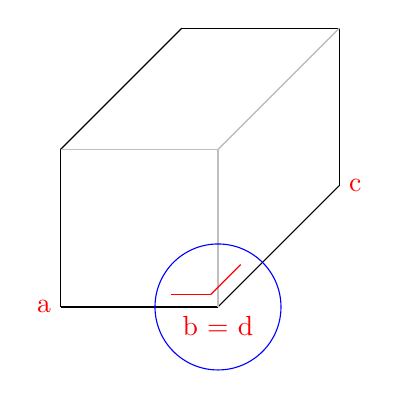
\begin{tikzpicture}
	\draw[black] (0,0 ,4) node[red,left]{a} -- (2,0,4);
    \draw[black] (0 ,0,4) -- (0 ,2,4);
    \draw[black] (2,0 ,4) -- (2,0 ,0);
    \draw[black] (0 ,2,4)  -- (0 ,2,0);
    \draw[black] (2,0,0 ) node[red,right]{c} -- (2,2,0 ) ;
    \draw[black] (0,2,0 ) -- (2,2,0 );
    
    \draw[lightgray] (0,2 ,4) -- (2,2 ,4);
    \draw[lightgray] (2 ,0,4) -- (2 ,2,4);
    \draw[lightgray] (2,2 ,4) -- (2,2 ,0);
    \draw[lightgray] (2 ,2,4) -- (2 ,2,0);
    \draw[lightgray] (2,0,4 ) -- (2,2,4 );
    \draw[lightgray] (0,2,4 ) -- (2,2,4 );
    
	\draw[red] (1.75,0 ,3.6) -- (1.25,0 ,3.6);
	\draw[red] (1.75,0 ,3.6) -- (1.75,0 ,2.6);
	
	\draw[blue] (2,0,4) node[red,below]{b = d}circle (0.8);
  \end{tikzpicture}
  \caption{Twee voorbeelden die aangeven hoe de pose vanuit een contour gevonden kan worden. }
  \label{fig:brickPoseDetect}
\end{figure}

Nu de contour is gevonden moet hieruit worden achterhaald wat de pose van de legoblok is, hiervoor bepalen we eerst in welk vlak van de legoblok elk hoekpunt van de contour ligt: onder- of bovenvlak. Dit geeft ons de $Z$ co\"ordinaat van al deze hoekpunten waardoor ze kunnen worden omgezet van 2D naar 3D via het pinhole model. Bij uitbreiding zijn dan alle hoekpunten van de legoblok in 3D gekend en dus kennen we ook de pose van de legoblok.

Eerst leggen we uit hoe kan achterhaald worden in welk vlak (boven of onder) elk hoekpunt van de contour ligt. Deze redenering wordt verduidelijkt met twee voorbeelden in figuur \ref{fig:brickPoseDetect}, waarin legoblokjes worden getoond met hun contourlijnen aangeduid in zwart.

Uit de geometrische informatie van een legoblok is geweten dat minstens drie opeenvolgende hoekpunten in hetzelfde Z-vlak liggen. Om te bepalen welke drie hoekpunten dit zijn zetten we alle 2D contourpunten om naar 3D (geprojecteerd op vlak $Z = 0$) en bepalen we welke drie opeenvolgende 3D hoekpunten ($a$, $b$ en $c$) een hoek vormen die het dichtst bij 90 graden ligt. Van deze hoeken zijn we dan zeker dat ze in hetzelfde vlak liggen. In het eerste voorbeeld van figuur \ref{fig:brickPoseDetect} ligt de hoek tussen drie hoekpunten in het bovenvlak dichtst bij 0, in het tweede voorbeeld is dit de hoek in het ondervlak. Een ander geval is onmogelijk omdat, na projectie op het ondervlak, hoeken tussen punten in een verschillend $Z$-vlak sterker zullen afwijken van 90 graden.

Vervolgens bepalen we het hoekpunt ($d$) dat in 3D (geprojecteerd op vlak $Z = 0$) zich het dichtst bij de camera bevindt, hiervan kan met zekerheid gezegd worden dat het werkelijk in het vlak $Z = 0$ ligt. Dit hoekpunt is in de voorbeelden aangeduid met een blauwe cirkel. Nu kan met zekerheid gezegd worden of $a$, $b$ en $c$ in het onder- of bovenvlak van de legoblok liggen: 
\begin{itemize}
\item Als $d == a$ $OF$ $d == b$ $OF$ $d == c$, dan liggen $a$, $b$ en $c$ in het ondervlak;
\item Anders liggen $a$, $b$ en $c$ in het bovenvlak.
\end{itemize}
In het eerste voorbeeld van figuur \ref{fig:brickPoseDetect} liggen de hoekpunten $a$, $b$ en $c$ dus in het bovenvlak aangezien hoekpunt $d$ niet gelijk is aan \'e\'en van deze hoeken. In het tweede voorbeeld is dit wel het geval en dus liggen de drie punten in het ondervlak. Dit geeft ons (via het pinhole model) de 3D posities van alle hoekpunten van de contour en bij uitbreiding van de volledige legoblok.

Ten slotte kunnen nog de afmetingen en precieze positie van de blok worden bepaald. In plaats deze informatie uit slechts \'e\'en frame te halen, wordt het achterhaald via een voting systeem over meerdere frames. Dit helpt om fouten in de vorige stappen van het algoritme te verkleinen. Het voting systeem werkt als volgt: 

De blok wordt in verschillende frames gedetecteerd en wanneer alle hoekpunten dichter dan 0.8 cm bij elkaar liggen wordt dit gezien als dezelfde blok. In dat geval kan gestemd worden op de grootte en positie van de blok door het gemiddelde te nemen van de groottes en posities van alle blokken die zo dicht bij elkaar liggen. De waarde 0.8 cm is niet toevallig gekozen: het is exact de helft van de breedte van een 2x2 legoblok, zo dicht kunnen legoblokken dus nooit bij elkaar liggen.

Bovendien kan een legoblok nog in een verschillende state verkeren om te bepalen wanneer de blok een deel van het spel wordt (\textit{actief}) en wanneer de blok er geen deel meer van uitmaakt (\textit{inactief}): Wanneer een blok minstens in drie frames werd gedetecteerd wordt hij actief, maar indien hij minstens drie frames achter elkaar niet werd gedetecteerd wordt hij inactief en wanneer hij na vijf frames achter elkaar niet is gedetecteerd wordt hij zelfs verwijderd. Dit mechanisme maakt het algoritme flexibeler om blokken te kunnen toevoegen of verwijderen uit het spel wanneer de speler dat wil.

\subsection{Resultaten en performantie} \label{sec:algo1_res}

\subsubsection*{Resultaten}

\begin{figure}
  \centering
  \includegraphics[width=\linewidth]{img/alg1}
  \caption{Resultaat van het eerste na\"ieve algoritme.}
  \label{fig:result_algo1}
\end{figure}


Figuur \ref{fig:result_algo1} toont het resultaat van het algoritme. De linkerafbeelding toont de legoblokken en de rechterafbeelding wat de detectie van legoblokken oplevert. 

Merk op dat de rendering van de gedetecteerde legoblokken een kleine afwijking bevat van de werkelijke legoblokken. Dit wordt veroorzaakt door een trage performantie van het algoritme, waardoor de rendering in feite van enkele frames geleden.

Verder valt ook op te merken dat de virtuele legoblokken iets groter zijn dan de werkelijke legoblokken. Dit was nodig omdat de virtuele wereld in feite bestaat uit een discreet grid. Om er zeker van te zijn dat de lemmings niet gedeeltelijk in een legoblok wandelen worden ze iets groter gemaakt dan hun werkelijke grootte.

\begin{figure}
  \centering
  \includegraphics[width=\linewidth]{img/alg1Shadow}
  \caption{Resultaat van het eerste na\"ieve algoritme bij veel schaduw.}
  \label{fig:algo1_shadow}
\end{figure}

In figuur \ref{fig:algo1_shadow} wordt aangetoond dat schaduw een negatief effect heeft op het resultaat van het algoritme. We zien in de threshold dat er wat artefacten op de plaats van de schaduw aanwezig zijn, dit resulteert uiteindelijk in legoblokken die moeilijk worden gevonden.

\begin{figure}
  \centering
  \includegraphics[width=\linewidth]{img/alg1NonWhiteBg}
  \caption{Resultaat van het eerste na\"ieve algoritme bij rode tint in het beeld.}
  \label{fig:algo1_nonwhitebg}
\end{figure}

Zoals aangegeven in sectie \ref{sec:alg1_begrip} is een rode tint in het beeld is absoluut uit den boze, elke kleur in het beeld dat een beetje in de grenzen van de threshold valt vormt een probleem. Dit tonen we aan in figuur \ref{fig:algo1_nonwhitebg}, waarin een bruine achtergrond in beeld komt. We zien duidelijk dat veel ruis in de threshold voorkomt. Het gevolg hiervan is vooral dat het algoritme enorm veel trager is dan normaal: soms duren alle berekeningen samen wel tot 5 seconden. Dit komt omdat ruis in de threshold het algoritme doet denken dat op die plaatsen ook legoblokken staan en daardoor zal het al die contouren ook willen verwerken wat veel tijd vraagt. Dit is natuurlijk onaanvaardbaar voor een spel met AR. Bovendien gebeurde het zelden wel eens dat de camera zelfs zijn belichting aanpaste (bijvoorbeeld wanneer plots grote hoeveelheden donkere kleuren in beeld komen), hierdoor werd de threshold voor de legoblok zelf ook slechter wat ertoe leidde dat de blok helemaal niet meer gedetecteerd werd.

\subsubsection*{Performantie}

\begin{figure}
  \centering
  \includegraphics[width=.75\linewidth]{img/alg1Perf}
  \caption{Gemiddelde performantie van het eerste na\"ieve algoritme.}
  \label{fig:perf_algo1}
\end{figure}

Figuur \ref{fig:perf_algo1} toont de performantie van het eerste na\"ieve algoritme voor de simpele scene (links) en complexe scene (rechts). De gele blok stelt telkens de totale tijd die het algoritme nodig heeft, de gekleurde blokken geven de onderverdelingen aan van deze tijd: 
\begin{itemize}
\item YUV omzetten naar BGR;
\item Camerapose berekenen (via markers);
\item Threshold berekenen en contouren van legoblokken zoeken (eerste deel van dit algoritme);
\item Pose van de blokken zoeken (tweede deel van dit algoritme);
\item Blokken toevoegen aan de virtuele wereld, mergen van blokken en voten voor grootte en positie van blokken.
\item Lemmings updaten (oa. pad van de lemming updaten).
\end{itemize}
Merk op dat de som van de gekleurde blokken niet exact gelijk is aan de grootte van de gele blok. Dit komt omdat enkel de belangrijkste onderdelen uit het algoritme zijn opgenomen in deze grafiek, enkele implementatie specifieke details zijn weggelaten omdat ze erg weinig tijd innemen en onbelangrijk zijn.

Uit de figuur kunnen we vooral opmaken dat het gedeelte van het zoeken van de contouren en zoeken van de pose erg veel verschillen tussen de complexe en simpele scene. Dit is normaal aangezien het aantal legoblokken hoger ligt en dus moet dit na\"ieve algoritme veer iteraties doen in een complexe scene.

We merken ook op dat het updaten van de lemmingen een stuk langer duurt, dit is ook aannemelijk omdat bij de complexe scene het pad van een lemming van begin tot eindpunt een stukje langer is dan bij de simpele scene. Aangezien dit pad ook steeds opnieuw wordt berekend (om \textit{on-the-fly} toevoegen van blokken toe te kunnen staan) is dit verschil significant.

Als we even kijken naar de totale tijd de volledige berekening inneemt, dan zien we toch dat dit algoritme erg traag is. Dit komt neer op een 5-tal fps voor de simpele scene en 1.8 fps voor de complexe scene, wat natuurlijk erg traag is voor een AR spel.

\subsection{Voor- en nadelen}
Deze na\"ieve implementatie heeft enkele voordelen:
\begin{itemize}
\item Ze laat toe dat legoblokken \textit{on-the-fly} worden toegevoegd aan de virtuele wereld.
\end{itemize}
Aan deze methode zijn echter heel wat nadelen verbonden:
\begin{itemize}
\item Legoblokken mogen niet in een hoek naast elkaar staan omdat dan de veronderstelling dat een contour maximaal zes hoeken bevat niet meer geldig is.
\item Enkel rode legoblokken kunnen worden gedetecteerd. Dit nadeel is echter eenvoudig weg te werken zoals wordt besproken in sectie \ref{sec:algo_grid}.
\item Legoblokken mogen niet in meerdere niveau's gebouwd worden. Muren zouden in principe wel kunnen (ze hebben immers maximaal zes hoekpunten) maar dan moet op \'e\'en of andere manier de grootte van deze muur bepaald worden, dit wordt uitgebreider behandeld in hoofdstuk \ref{hoofdstuk:4}. Andere constructies in de hoogte kunnen echter niet vanwege dezelfde reden als het eerste nadeel.
\item Het algoritme kan niet goed om met veranderingen qua belichting. Dit komt omdat we puur thresholden op basis van kleur maar deze waarden zijn sterk afhankelijk van welke belichting we gebruiken. In hoofdstuk \ref{hoofdstuk:4} komt een calibratiemethode aan bod die dit probleem verhelpt.
\item Zoals aangegeven in de resultaten geeft een rode tint in het beeld een erg slecht resultaat, vooral qua performantie.
\item Performantie is erg laag.
\end{itemize}
 
\section{Blokdetectie met behulp van een 2D grid} \label{sec:algo_grid}
Dit algoritme is een sterke vereenvoudiging van het vorige. In plaats van werkelijk de pose en positie van de legoblok te bepalen, gebruiken we enkel de threshold. Eerst behandelen we de aanpassingen ten opzichte van het vorige algoritme en vervolgens bespreken we de gevolgen die deze aanpassingen hebben.

\subsection{Begrippen}
Deze sectie behandelt enkele nieuwe begrippen die in het algoritme worden gebruikt.

\textbf{Morphologische operaties} zijn operaties die de geometrie van vormen in een binaire afbeelding kunnen wijzigen. De twee basis operaties zijn \textit{dilate} en \textit{erode}. In deze operaties komt er op neer dat we de convolutie nemen van de afbeelding met een kernel, die eender welke vorm of grootte kan hebben. Hierbij wordt de kernel over de afbeelding geschoven en dan wordt de pixel in het ankerpunt van de kernel vervangen door een maximum of minimum van alle pixels die binnen de kernel vallen. Bij een \textit{dilate} operatie is dit het maximum en bij een \textit{erode} operatie is dit het minimum. Bij een \textit{dilate} en \textit{erode} operatie wordt een zwart vlak dus respectievelijk kleiner en groter. 

Naast de basis morphologische operaties bestaan ook nog de veel gebruikte \textit{open} en \textit{close} operatie. \textit{Open} is in feite een \textit{dilate} operatie toepassen op een afbeelding die eerder een \textit{erode} operatie onderging. De \textit{close} operatie is het omgekeerde. De \textit{open} operatie wordt vaak gebruik om kleine witte vlekjes te verwijderen, terwijl de \textit{close} operatie wordt gebruikt om kleine zwarte vlakjes te verwijderen.

\subsection{Algoritme}
Het eerste deel van het vorige algoritme wordt sterk ingekort aangezien we enkel een threshold nodig hebben. Maar er zijn ook een tweetal toevoegingen om tegemoet te komen aan de nadelen van het vorige algoritme:

Ten eerste berekenen we opnieuw een kleurenthreshold maar deze keer niet enkel voor de kleur rood, ook voor geel en blauw. Op die manier  willen we aantonen dat het algoritme zonder problemen met meerdere kleuren overweg kan. Dit zijn kleurengrenzen die werden gebruikt om in een HSV afbeelding te thresholden zodat het resultaat een afbeelding is waarin de legoblokken wit zijn en de achtergrond zwart:
\begin{align*}
Rood: 160 < H < 180; 153 < S < 255; 30 < V < 255 \\
Geel: 135 < H < 160; 147 < S < 255; 30 < V < 255 \\
Blauw: 0 < H < 112; 42 < S < 255; 13 < V < 255
\end{align*}

\begin{figure}
  \centering
  \includegraphics[width=0.5\linewidth]{img/alg2Noise}
  \caption{Ruis in threshold boor morphologische operaties.}
  \label{fig:algo2_noise}
\end{figure}

Ten tweede, omdat we nu thresholden op meerdere kleuren kan het gebeuren dat er wat ruis optreedt in onze threshold. Deze ruis vertoont zich in hoopjes witte of zwarte lijntjes op plaatsen waar het niet hoort (zie figuur \ref{fig:algo2_noise}). Om dit te vermijden worden de morphologische operaties \textit{open} en \textit{close} toegepast op de threshold.

Het tweede deel van het vorige algoritme ('het bepalen van de pose') valt volledig weg, logisch want we hebben geen contour bepaald. In plaats daarvan wordt het grid van onze virtuele wereld naar 2D omgezet (via het pinhole model). Dit 2 dimensionaal grid kunnen we vervolgens overlappen met de eerder berekende threshold en wanneer een gridnode zich in een witte regio van de threshold bevindt beschouwen we deze gridnode als 'bezet door een legoblok'.

\subsection{Gevolgen}
Dit algoritme is een grove versimpeling van het eerste algoritme aangezien de positie en grootte van een legoblok niet meer expliciet wordt bepaald. Nu vragen we ons af welke consequenties dat heeft.

\begin{figure}
  \centering
  \includegraphics[width=\linewidth]{img/alg2Shadow}
  \caption{Fout van dit algoritme in de vorm van schaduw.}
  \label{fig:algo2_shadow}
\end{figure}

Ten eerste wordt een fout gemaakt in het aantal gridnodes die bezet worden door een legoblokje. Deze fout wordt gemaakt omdat een onbezet deel schuilt achter de legoblok en dus niet zichtbaar is in een 2D camera frame. Sterker nog: we kunnen precies defini\"eren dat die fout even groot is als de schaduw op het grondvlak wanneer een lichtbron vanuit de camera schijnt in dezelfde richting als de camera kijkt. Afbeelding \ref{fig:algo2_shadow} toont de fout in de vorm van schaduw als de camera op de plaats van de lichtbron stond. We zien dat de fout relatief klein is wanneer de camera hoog boven het grondvlak staat (links) en groter wordt wanneer de camera dichter naar het grondvlak toe beweegt (rechts).

Ten tweede heeft dit algoritme ook een aantal voordelen in die zin dat enkele nadelen uit het vorige algoritme werden weggewerkt:
\begin{itemize}
\item Legoblokken in meerdere kleuren kunnen worden gebruikt, het gevolg is wel dat morphologische operaties de threshold moeten oppoetsen om er kleine foutjes uit te halen. Dit werd hoogstwaarschijnlijk veroorzaakt door de belichting die niet altijd constant is, zodat de thresholdwaarden niet altijd even nauwkeurig zijn. Merk op dat dit even goed in het eerste algoritme had kunnen worden ge\"implementeerd.
\item Legoblokken kunnen nu ook in een hoek tegen elkaar staan, wat bij het eerste algoritme niet was toegestaan. Een nadeel is echter wel dat meerdere niveau's in dit algoritme helemaal uitgesloten zijn, terwijl dit in het vorige algoritme, althans in theorie en met restricties, wel mocht. Dit komt omdat, als we de constructie hoger maken, dan de fout die we in dit algoritme maken steeds groter wordt. Er is immers een nog groter gedeelte van het grondvlak, waar geen legoblokken op staan, verborgen achter de legoblokconstructie.
\end{itemize}

\subsection{Resultaten en performantie}

\subsubsection*{Resultaten}
Voor dit algoritme is het niet mogelijk om een rendering te maken van de virtuele legoblok (zoals bij het eerste algoritme in sectie \ref{fig:result_algo1}). Dit komt omdat de legoblokken in principe nooit volledig worden berekend: enkel een threshold wordt gebruikt waar vervolgens een grid over wordt gelegd.

\begin{figure}
  \centering
  \includegraphics[width=.5\linewidth]{img/alg2}
  \caption{Resultaat van het tweede na\"ieve algoritme.}
  \label{fig:algo2_res}
\end{figure}

Figuur \ref{fig:algo2_res} toont het resultaat door het zwarte deel van de threshold deels transparant te maken. We kunnen duidelijk zien dat de legoblokken goed werden gedetecteerd via kleurthresholding. Ook werd over het grondvlak het grid gelegd, hierdoor is het duidelijk welke nodes niet toegankelijk zijn voor lemmings.

\subsubsection*{Performantie}
TODO: BESPREKING PERFORMANTIE

Omdat de performantie van dit algoritme erg laag is, aangezien we elke keer opnieuw een volledig pad moeten berekenen en dus ook veel gridnodes moeten omzetten van 3D naar 2D, gebruiken we in plaats van A* om paden te zoeken Tree Adaptive A*. In deze uitbreiding zullen grote delen van reeds berekende paden herbruikbaar zijn waardoor al deze gridnodes niet opnieuw van 3D naar 2D moeten worden omgezet.
 
\subsection{Uitbreiding: Tree Adaptive A*}

In deze sectie leggen we uit hoe Tree Adaptive A* (Tree-AA*) werkt en in welke mate het de performantie heeft verhoogd. Dit algoritme is in dieper detail uitgelegd in~\cite{hernandez2011tree}.

\subsubsection*{Algoritme}

\begin{figure}
  \centering
  \includegraphics[width=\linewidth]{img/TAAStar}
  \caption{Voorbeeld van het Tree Adaptive A* algoritme (uit~\cite{hernandez2011tree}).}
  \label{fig:taastar}
\end{figure}

Tree Adaptive A* is een algoritme dat een uitbreiding is op Path Adaptive A*, wat op zijn beurt een uitbreiding is op Adaptive A*. Het algoritme gaat uit van de \textit{freespace assumptie}, waarin een agent zich door een onbekend terrein een pad moet banen. Met een onbekend terrein bedoelen we dat hij de obstakels niet weet zijn, hij kan enkel obstakels om zich heen voelen. Hierdoor zal de agent elke keer hij een onbekend obstakel voelt het pad met optimale kost moeten aanpassen. Bij elke aanpassing mag de agent wel gebruik maken van de suffixen van vorige minimale kost paden (behalve natuurlijk de stukjes paden die door het obstakel gingen). De vorige paden die herbruikbaar zijn worden steeds opgeslagen in een datastructuur die de \textit{herbruikbare boom} wordt genoemd (het is namelijk een boom met zijn root in de doelcel). Zo moet de agent telkens slechts een deel van het pad aanpassen wat het zoeken van een pad een heel stuk effici\"enter maakt. De grootste kost zit dan in de initi\"ele zoektocht van een pad maar aangezien de meeste obstakels dan nog niet door de agent kunnen worden gezien zal dit best meevallen. 

We zetten onze uitleg nog kracht bij met het voorbeeld uit~\cite{hernandez2011tree} dat getoond wordt in figuur \ref{fig:taastar}. Alle grijze tegels zijn ge\"expandeerde nodes en de zwarte tegels zijn de obstakels waar de agent weet van heeft. Figuur \ref{fig:taastar}a toont het beginsituatie, figuur \ref{fig:taastar}b toont de situatie waarin gezocht wordt naar een pad met minimale kost tot de doelcel. Nog geen obstakels zijn gevonden omdat deze zich niet bevinden rondom de huidige cel van de agent. Het zoeken stopt wanneer men net cel D6 wil gaan expanderen, het resulterende pad is dan D1, D2, D3, D4, D5 en D6. De agent gaat dan naar cel D3 en voelt van daaruit een obstakel in cel D4. Dan wordt de het vorige minimale kost pad deels verwijderd. Hierdoor blijft het stukje tussen D5 en D6 over in de \textit{herbruikbare boom} omdat dit nog steeds deel kan uitmaken van een minimaal kost pad (we weten immers niet of op plaats D5 ook een obstakel zou liggen). De agent vindt vervolgens een nieuw pad dat ook aan de boom wordt toegevoegd. In de vierde stap wordt een obstakel ontdekt in cel C4 waardoor het stuk pad D3, C3, C4, C5 verdwijnt uit de boom terwijl het stukje C5, C6, D6 in de boom blijft. Bij het vinden van het nieuwe pad wordt het stukje C6, D6 herbruikt. Voor een meer gedetailleerde uitleg over het algoritme: zie paper~\cite{hernandez2011tree}.

Het grote voordeel aan dit algoritme voor een AR spel is dat deze \textit{herbruikbare boom} kan gedeeld worden tussen lemmingen. Dus als de wereld niet veranderd moeten weinig stukjes pad herberekend worden.


\subsubsection*{Performantie}

\section{Besluit van dit hoofdstuk}
%%% Local Variables: 
%%% mode: latex
%%% TeX-master: "masterproef"
%%% End: 
